
\documentclass[a4paper,12pt,twoside]{exam}
\usepackage{acn-particlestyle}
\usepackage{acn-scientific}
\usepackage{acn-questions}

\usetikzlibrary{circuits.ee.IEC}

\usepackage{color}
\definecolor{heberblue}{rgb}{0,0,1}

\newcounter{saveenumi}


\begin{document}

\begin{titlepage}

\begin{minipage}{0.2\textwidth}
\includegraphics[width=0.8\textwidth]{img/heber.jpg}
\end{minipage}
\hspace{0.05\textwidth}
\begin{minipage}{0.7\textwidth}
\begin{Huge}\textcolor{heberblue}{\textbf{Bishop Heber High School}}\end{Huge}
\end{minipage}\\

\bfseries

\vspace{6em}

\begin{Huge}Practical Physics I\end{Huge}\\
\indent \Large Lower Sixth\\

Autumn term 2013\\


\begin{minipage}{0.45\textwidth}
\hfill
\includegraphics[width=0.9\textwidth]{img/positrondiscovery.jpg} 
\hfill	
\end{minipage}
\begin{minipage}{0.45\textwidth}
\footnotesize{{
The discovery photograph of the positron, the positive version of the electron and the first antimatter particle to be discovered. The cloud chamber photo was taken in 1932 by US physicist Carl Anderson. It shows the track of a positive particle that enters the chamber from below. The particle is known to be positive because of the way it bends in the chamber's magnetic field; it is known to be moving up the picture because it loses energy and so curves more in the magnetic field after traversing the \SI{6}{mm} thick lead plate in the middle. The track is too faint to be caused by a proton---it is exactly like an electron's track---and so it had to be the predicted positron.
}}
\end{minipage}
\begin{flushright}
\rmfamily{\small{CARL ANDERSON / SCIENCE PHOTO LIBRARY}}
\end{flushright}

\vfill

\begin{minipage}{0.5\textwidth}
Name:\\
\hrule
\vspace{0.5em} Form: \\
\hrule
\vspace{0.5em} Set: \\
\hrule
\end{minipage}

\thispagestyle{empty}
%\enlargethispage{4cm}
	
\end{titlepage}

\newpage
\thispagestyle{empty}

\vspace*{4cm}

\begin{center}
\fbox{
\begin{minipage}{0.65\textwidth}
\vspace*{1em}
\begin{center}
\includegraphics[width=0.3\textwidth]{by-nc-sa.png}
\end{center}
\raggedright

This work by A.C. Norman is licensed under a Creative Commons
Attribution-NonCommercial-ShareAlike License.

{\footnotesize\texttt{http://creativecommons.org/licenses/by-nc-sa/3.0/}}\\

\vspace{1em}

Non-commercial uses are thus permitted without any
further permission from the copyright owner.\\

\vspace{1em}

%Permissions beyond the scope of this license are
%administered by the author. Information on how
%to request permission may be found at:
%http://www.randomhouse.com/about/
%permissions.html
\end{minipage}
}
\end{center}

\newpage


\section*{Errors}

In practical work in AS and A2 physics, you should be prepared to
\begin{itemize}
\item identify the source of uncertainties in an experiment.
\item calculate the fractional or percentage error from the size of the measurement and the absolute error on it.
\item combine the uncertainties of different measurements when you evaluate something which depends on a number of quantities. It is very unlikely that you will have to do a full calculation of the total error, but you may be asked, for example, to identify which individual measurement contributes the biggest uncertainty.
\end{itemize}

\subsection*{Sources of uncertainty and absolute errors}

Any measurement has a statistical uncertainty associated with it. It is generally a combination of both the reading error on a measuring instrument and the uncertainty to do with the way you are performing the measurement. For example, the reading error on a \SI{1}{m} ruler is at best \SI{0.5}{mm}. If you are using it to measure the depression of another ruler, you might reasonably assign a total uncertainty of \SI{3}{mm}, to account for the fact that you may not have the measuring ruler absolutely vertical. An error of this kind is an absolute error, and has the dimension of the quantity you are measuring.

Systematic errors may also be built in to the experiment, for example the ruler above may have an actual length of say \SI{99}{cm} when you have assumed to be \SI{1}{m}, or an ammeter may show a non-zero reading when disconnected from an electric circuit. Such uncertainties may not alter the reliability of your readings, but they may well affect the accuracy of a calculated quantity.

\subsection*{Fractional or percentage errors}

These are dimensionless and are calculated using the formula
\[\text{fractional error} =  \frac{\text{absolute error}}{\text{size of measurement}}.\]

\subsection*{Combination of errors}

\begin{itemize}
\item If you make two measurements of the same type $x$ and $y$, for example the length and breadth of a table, then
absolute error on the sum $x+y$ or difference $x-y$ of $x$ and $y$ is equal to the sum of absolute errors on $x$ and $y$.
\item If you make measurements of any two quantities $x$ and $y$, then 
fractional error on the product $xy$ or quotient $x/y$ is equal to the sum of fractional errors on $x$ and $y$.
\item If a power law holds
\[\text{fractional error on $x^{k}$}  = k \times \text{fractional error on $x$}.\]
\end{itemize}

%Example 1 . A rectangular table is measured to have length 2.5m � 2mm and breadth 0.5m � 2mm. Find the absolute error on the %circumference and the area.

%Answer	Absolute error on circumference = sum of absolute errors on four sides = 4 ? 2mm = 8mm
%Fractional error on area = 
%fractional area on length + fractional area on breadth = 2mm/2.5m +  2mm/0.5m =  0.5 %.
%Absolute error on area = 0.5 % ? (2.5 m ? 0.5 m) =  60 cm2.

%Example 2. A simple pendulum is measured to be 50cm � 5mm in length. Ten swings are timed to take 14.0 s � 0.2s. Which measurement contributes a larger uncertainty to a value of g derived from this experiment ?  What is the absolute error on g? 

%Answer	T = 2??(l/g) therefore g = 4?2l/T2.   
%Fractional error on g = 
%fractional error on l + 2 ? fractional error on T = 0.5/50  + 2 ? 0.02/1.40 = 1% + 3% = 4%.
%Therefore the error on the period has a far greater contribution than that on the length. Note that if only one swing was timed, the fractional error on the period would be ten times as large.
%Absolute error on g = fractional error ? size of g = 4% ? 10.1 ms-2   =  0.4 ms-2. 
%Although the value of g is greater than the true value of 9.81 ms-2, the measurement is in agreement within the error, as it should be if the errors have been realistically assessed. 

%Error on a count

%Any count of a number of occurrences e.g. the number of clicks of a Geiger counter in a period of time has an uncertainty associated with it. If there are N counts, then the absolute error is of size ?N. Thus the absolute error increases with N, but the fractional error =   ?N / N = 1/?N gets smaller. Therefore it is desirable to make the number of counts as big as possible.
%E.g. if a Geiger counter records 100 background counts over a period of 1 minute, the percentage error is 100% ? (1/?100) = 10%. 
%If the same measurement is made over 4 minutes, we expect a percentage error of 100% ? (1/?400) = 5%.

\newpage
\section*{Determining relationships by plotting graphs}

When a certain relationship exists between two variables $y$ and $x$, its form can sometimes be determined by plotting a suitable graph. You should be familiar with the following cases.

\subsection*{Linear}

If $y = mx + c$ a graph of $y$ against $x$ should be a straight line with gradient $m$ and $y$-intercept $c$.\\
NB $y$ is only proportional to $x$ if $c = 0$.

\subsection*{Exponential}

If  $y = Ae^{-mx}$ , where $A$ is a constant, then taking natural logs of both sides gives
\[ \ln y = \ln A + \ln(e^{-mx}) = \ln A - mx.\]
Hence a graph of $\ln y$ against $x$ should be a straight line of gradient $-m$ and intercept $\ln A$.\\
Examples of such relationships are found in radioactive decay and in electric circuits containing capacitors.

\subsection*{Polynomial}

If  $y = Ax^{m}$  , then taking natural logs of both sides gives
 \[\ln y = \ln A + \ln(x^{m}) = \ln A +  m\ln x.\]
Hence a graph of $\ln y$ against $\ln x$ should be  a straight line of gradient $m$ and intercept $\ln A$.\\
Examples include the variation of the period of a simple pendulum with length ($m = 0.5$) and the energy stored in a stretched spring with extension ($m = 2$).

\section*{Errors obtained from graphs}

When it is believed that a linear relationship exists between two quantities plotted on a graph, a straight line of best fit should be drawn through the points, which passes as close to all the points as possible. 

You can draw error bars for each point so that the length of the line on either side of the point represents the absolute error you have assigned to the individual measurements. The line of best fit should pass through about two-thirds of the error bars, if you have assessed the errors realistically (and if a linear relationship holds).

It is common to extract the gradient or the intercept since they often correspond to something interesting. You can evaluate the error on them by drawing another fit line, making it as steep or shallow as possible, so that it still passes through the error bars. The difference between the values so obtained for the gradient and intercept, and those of the best-fit line correspond to the absolute errors.


\newpage
\section*{Index}
%\setlength{\extrarowheight}{0.3cm}
\renewcommand{\arraystretch}{2}
\begin{center}
\begin{tabular}{|l|c|p{2.5cm}|p{2cm}|c|}
\hline
\multicolumn{1}{|c|}{\bf Experiment} & \multicolumn{1}{|c|}{\bf Page} & \multicolumn{1}{|c|}{\bf Date} & \multicolumn{1}{|c|}{\bf Mark}\\
\hline
\ref{ivchar} - $I-V$ characteristics & \pageref{ivchar} & & \\
\hline
\ref{intres} - Internal Resistance & \pageref{intres} & & \\
\hline
\ref{resistivity} - Resistivity of a wire & \pageref{resistivity} & &\\
\hline
\ref{planck} - Planck's Constant & \pageref{planck} & & \\
\hline
\ref{photoelectric} - Photoelectric effect & \pageref{photoelectric} & & \\
\hline
\ref{tracks} - Particle tracks & \pageref{tracks} & &\\
\hline
\ref{bubble} - Bubble chamber & \pageref{bubble} & &\\
%\hline
%\ref{electron} - Electron specific charge & \pageref{electron} & &\\
%\hline
%\ref{gamma} - $\gamma$ absorption & \pageref{gamma} & &\\
%\hline
%\ref{decay} - Radioactive decay & \pageref{decay} & & \\
\hline
\end{tabular}
\end{center}

\section*{Writing up A-level practicals}

During your practical lessons over the next year or two we require you to perform the practical, produce some results, and do some processing of the data.  Possibly even evaluating a quantity which appears to have no relevance!  You will then usually answer some questions relating to possible errors.

The aims of the experiments are to supplement the theory taught in lessons, to give you some insight into experimental physics and also to help you to develop skills which will help you in the practical examination.  We have tried to make this workbook fairly complete, and you will not usually need to make copious notes or draw diagrams.  You will simply answer the questions asked by filling in the blanks in this booklet.  Since the demands on you in this respect are relatively low, we do demand high standards from you. Please take care and learn from your mistakes--do not simply glance at the mark you have gained from the previous practical (instead, see where you dropped marks, and ensure you do not repeat these errors).

The apparatus in the actual practical examination will be set up for you ready to use.  In the lessons, we do not have the time to do this, and you will have to set up the apparatus yourself (and put it away properly for the next person to use!)  We need you to fill in the index above each week with the date on which you did a particular practical and after marking we shall insert a mark for it.

You will be marked on the following points, if applicable:
\begin{itemize}
\setlength{\itemsep}{1pt}
  \setlength{\parskip}{0pt}
  \setlength{\parsep}{0pt}
\item Results table (probably in columns) with headings including appropriate unit
\item All figures to an appropriate accuracy, probably 3 s.f.
\item Graphs with appropriate scales (no scales of 3, cannot be doubled and still fit on axis). Minimum acceptable size: $\SI{8}{cm}\times\SI{8}{cm}$
\item Accuracy of point plotting from results table, appropriate line of best fit
\item LARGE gradient triangle shown on graph, length of $\Delta y$ and $\Delta x$ marked on with units
\item Gradient calculation must be shown $(\Delta y/\Delta x)$ including units throughout, NB some may be negative
\item Estimated of possible errors in quantities, BE REALISTIC
\item Your answers on how to reduce errors, how you ensured accuracy in your experiment
\end{itemize}

We want you to enjoy practical work but also ensure you are continually improving since it is a very important skill and furthermore a rich source of very straightforward marks!

\normalsize

\cleardoublepage

\section{$I-V$ characteristics}
\label{ivchar}

This practical comprises three related experiments, which will allow you to plot $I-V$ graphs for an ohmic conductor, a filament lamp, and a diode.

Set up the circuit as shown below, noting the following points:
\begin{itemize}
\item Place the components in the board as shown, with the ohmic conductor (resistor) as the first component
\item The ammeter is to be set on the \SI{200}{mA} range
\item the voltmeter is to be set on the 2V range
\item Set the power supply voltage to about \SI{4}{V} d.c. making sure the positive and negative are as shown
\end{itemize}

\begin{center}
\begin{tikzpicture}[circuit ee IEC]
%power supply + rheostat slide
\draw (0,0) node[contact]{} node[anchor=east]{\SI{0}{V}} to (1,0) to [resistor] (1,5) to (0,5) node{} node[anchor=east]{+\SI{4}{V}} node[contact]{};
%bottom rail
\draw (0,0) to (11,0);
%right end
\draw (11,0) to [circuit handle symbol={draw,shape=circle,label=center:{V},minimum size=10mm}] (11,5);
%pot +top rail
\draw (2,2.5) to (2,5) to [circuit handle symbol={draw,shape=circle,label=center:{A},minimum size=10mm}] (8,5) to (11,5);
\draw[->] (2,2.5)--(1.2,2.5);
%contacts:
\draw (8,0) to (8,2) node[contact]{};
\draw (8,5) to (8,3) node[contact]{};
\draw (8,2.5) node {component};
\end{tikzpicture}
\end{center}

\begin{questions}
\question Using the variable resistor (and if necessary the voltage setting on the power supply), measure the current through  the ohmic conductor for voltages between \SI{0.00}{V} and \SI{0.60}{V}, ion \SI{0.10}{V} steps.

\begin{center}
\begin{tabular}{|c|c|}
\hline
Voltage $V$ / V & Current $I$ / mA\\
\hline 
& \\
\hline
& \\
\hline
& \\
\hline
& \\
\hline
& \\
\hline
& \\
\hline
& \\
\hline
\end{tabular}
\end{center}

\newpage

\question Replace the ohmic conductor with the filament lamp, and repeat the experiment.

\begin{center}
\begin{tabular}{|c|c|}
\hline
Voltage $V$ / V & Current $I$ / mA\\
\hline 
& \\
\hline
& \\
\hline
& \\
\hline
& \\
\hline
& \\
\hline
& \\
\hline
& \\
\hline
\end{tabular}
\end{center}


\question Replace the filament lamp withthe diode. \textbf{Make sure that the diode is forward biased}, i.e. it faces in the direction of conventional current flow.  Repeat the experiment, however this time increase the p.d. in steps of \SI{0.10}{V} until \SI{0.5}{V}, noting the current, then continue by increasing the current in steps of \SI{20.0}{mA}, noting the voltage.

\begin{center}
\begin{tabular}{|c|c|}
\hline
Voltage $V$ / V & Current $I$ / mA\\
\hline 
0.00 & \\
\hline
0.10 & \\
\hline
0.20 & \\
\hline
0.30 & \\
\hline
0.40 & \\
\hline
0.50 & \\
\hline
& 20.0\\
\hline
& 40.0\\
\hline
& 60.0\\
\hline
\end{tabular}
\end{center}

\question Plot a graph of $I$ on the $y$-axis against $V$ on the $x$-axis for each component \textbf{using the same scales (but different axes) for all.}


\newpage
\thispagestyle{empty}
\begin{tikzpicture}[remember picture, overlay]

\tikzset{normal lines/.style={gray, very thin}} 
\tikzset{margin lines/.style={gray, thick}} 
\tikzset{mm lines/.style={gray, ultra thin}} 
\tikzset{strong lines/.style={black, very thin}} 
\tikzset{master lines/.style={black, very thick}} 
\tikzset{dashed master lines/.style={loosely dashed, black, very thick}} 

\node at ([xshift=1cm, yshift=8.5mm] current page.south west){
  \begin{tikzpicture}[remember picture, overlay]

    \draw[style=mm lines,step=1mm] (0,0) grid +(19cm,28cm); 
    \draw[style=strong lines,step=1cm] (0,0) grid +(19cm,28cm); 

  \end{tikzpicture}
};
\end{tikzpicture}


\newpage
\thispagestyle{empty}
\begin{tikzpicture}[remember picture, overlay]

\tikzset{normal lines/.style={gray, very thin}} 
\tikzset{margin lines/.style={gray, thick}} 
\tikzset{mm lines/.style={gray, ultra thin}} 
\tikzset{strong lines/.style={black, very thin}} 
\tikzset{master lines/.style={black, very thick}} 
\tikzset{dashed master lines/.style={loosely dashed, black, very thick}} 

\node at ([xshift=1cm, yshift=8.5mm] current page.south west){
  \begin{tikzpicture}[remember picture, overlay]

    \draw[style=mm lines,step=1mm] (0,0) grid +(19cm,28cm); 
    \draw[style=strong lines,step=1cm] (0,0) grid +(19cm,28cm); 

  \end{tikzpicture}
};
\end{tikzpicture}

\newpage
\question \begin{parts} 
\part Calculate the gradient of the graph for the ohmic conductor

\fillwithlines{3cm}

\part The resistance of the ohmic conductor is given by the reciprocal of this gradient.  Calculate the resistance of the ohmic conductor.

\fillwithlines{2cm}

\part Using values from you table, calculate the resistance of the filament lamp for two different calues of voltage.

\fillwithlines{2cm}

\part Explain why the resistance of the filament lamp changes in this way.

\fillwithlines{3cm}

\part Explain the shape of the diode graph in terms of its resistance.

\fillwithlines{3cm}

\part What would the graph for the diode look like if it were to be placed in the reverse direction?

\fillwithlines{3cm}

\end{parts}

\end{questions}
%graph paper incl.

\cleardoublepage

\section{Internal Resistance}
\label{intres}
%NB this is closely based on the AQA June 2009 ISA

In this experiment you are going to carry out an experiment to investigate the relationship between the potential difference across the terminals of a \SI{1.5}{V} `AA' battery and the current through it.

You will use several different resistors, each of which will draw a different current through the battery.

\begin{questions}
\question Set up the circuit as show in the diagram below, using the \SI{22}{\ohm} resistor.
\begin{center}
\begin{tikzpicture}[circuit ee IEC]
%top rail with battery
\draw (0,5) to [battery] (8,5);
%left side and resistor
\draw (0,5) to (0,0) to [resistor] (8,0);
%right side with ammeter
\draw (8,0) to [circuit handle symbol={draw,shape=circle,label=center:{A},minimum size=10mm}] (8,5);
%voltmeter
\draw (2,5) to (2,3) to [circuit handle symbol={draw,shape=circle,label=center:{V},minimum size=10mm}] (6,3) to (6,5);
%labels
\draw (4,-0.5) node {\SI{22}{\ohm}};
\draw (4,5.5) node {\SI{1.5}{V} `AA' battery};
\end{tikzpicture}
\end{center}

\question Record the current shown on the ammeter. \answerline

\question What is the precision of the ammeter? \answerline

\question Using the instrument precision, work out the percentage uncertainty in the ammeter reading.
\fillwithlines{2cm}

\question Explain why using resistors with very high values would be unsuitable in this experiment.
\fillwithlines{3cm}

\newpage

\question Substituing each resistor into the circuit in turn---start by replacing the \SI{22}{\ohm} resistor with the \SI{10}{\ohm} resistor---record the values of the current and terminal p.d. in the table below.  \emph{Make sure you disconnect the battery between readings.}

\begin{center}
\begin{tabular}{|c|c|c|}
\hline
Resistor value / \si{\ohm} & Current $I$ / mA & Terminal p.d. / V\\
\hline 
22 & & \\
\hline
10 & & \\
\hline
6.8 & & \\
\hline
4.7 & & \\
\hline
3.3 & & \\
\hline
2.2 & & \\
\hline
1.5 & & \\
\hline
1.0 & & \\
\hline
\end{tabular}
\end{center}

\question Plot a graph of terminal p.d. on the $y$-axis against current $I$ on the $x$-axis.

The equation relating terminal p.d. $V$ and current $I$ is
\[V = \epsilon - Ir,\]
where $\epsilon$ is the emf of the supply and $r$ is the internal resistance of the supply.

\question By reference to the equation of a straight line $y = mx + c$,
\begin{parts}
\part what physical quantity is represented by the intercept on the p.d. axis?
\fillwithlines{1cm}
\part what physical quantity is represented by the gradient of the graph?
\fillwithlines{1cm}
\end{parts}

\question Use a line of best fit to help you to determine the emf and the internal resistance of the battery in this experiment, showing your working clearly.
\fillwithlines{5cm}

\newpage
\thispagestyle{empty}
\begin{tikzpicture}[remember picture, overlay]

\tikzset{normal lines/.style={gray, very thin}} 
\tikzset{margin lines/.style={gray, thick}} 
\tikzset{mm lines/.style={gray, ultra thin}} 
\tikzset{strong lines/.style={black, very thin}} 
\tikzset{master lines/.style={black, very thick}} 
\tikzset{dashed master lines/.style={loosely dashed, black, very thick}} 

\node at ([xshift=1cm, yshift=8.5mm] current page.south west){
  \begin{tikzpicture}[remember picture, overlay]

    \draw[style=mm lines,step=1mm] (0,0) grid +(19cm,28cm); 
    \draw[style=strong lines,step=1cm] (0,0) grid +(19cm,28cm); 

  \end{tikzpicture}
};
\end{tikzpicture}


\newpage
\thispagestyle{empty}
\begin{tikzpicture}[remember picture, overlay]

\tikzset{normal lines/.style={gray, very thin}} 
\tikzset{margin lines/.style={gray, thick}} 
\tikzset{mm lines/.style={gray, ultra thin}} 
\tikzset{strong lines/.style={black, very thin}} 
\tikzset{master lines/.style={black, very thick}} 
\tikzset{dashed master lines/.style={loosely dashed, black, very thick}} 

\node at ([xshift=1cm, yshift=8.5mm] current page.south west){
  \begin{tikzpicture}[remember picture, overlay]

    \draw[style=mm lines,step=1mm] (0,0) grid +(19cm,28cm); 
    \draw[style=strong lines,step=1cm] (0,0) grid +(19cm,28cm); 

  \end{tikzpicture}
};
\end{tikzpicture}

\newpage
\question Why do you think you were instructed to switch off or disconnect the battery between readings?
\fillwithlines{2cm}

\question Do you think your readings are reliable? Give a reason for your answer.
\fillwithlines{2cm}

\question The manufacturer quotes the resistors used as having an uncertainty (the
manufacturer's `tolerance') of 5\% . 
\begin{parts}
\part Calculate the maximum possible value of the \SI{6.8}{\ohm} resistor used in this experiment. \answerline
\part Explain why it would not have made any difference to the value of  obtained in the
experiment if resistors with a tolerance of only 2\%\ had been used instead.
\fillwithlines{2cm}
\end{parts}

\question The voltmeter used in the above experiment was found to have a calibration error
whereby every reading was \SI{0.22}{V} too high.
\begin{parts}
\part What is the name given to this type of error?
\fillwithlines{1cm}
\part How, if at all, would this have affected the value obtained for the intercept of the graph?
\fillwithlines{2cm}
\part How, if at all, would this have affected the value for the gradient of the graph?
\fillwithlines{2cm}
\end{parts}

\end{questions}


\cleardoublepage

\section{Resistivity of a wire}
\label{resistivity}

\begin{questions}
\question 
\begin{parts}
\part Using the micrometers, measure the diameter of the wire at three different points, and calculate $d$, the average diameter\\

\noindent\begin{tabular}{|p{2cm}|p{2cm}|p{2cm}|p{2cm}|}
\hline
$d_{1}/\si{mm}$ & $d_{1}/\si{mm}$ & $d_{1}/\si{mm}$ & $d/\si{mm}$\\
\hline
&&&\\
\hline
\end{tabular}\\
\part Calculate the average cross-sectional area of the wire, $A$, in \si{m^2}.
\fillwithlines{1cm}
\end{parts}
\question Set up the circuit as shown below, noting the following points:
\begin{itemize}
\item Set the length of the wire between the crocodile clips, $l$, to be \SI{1.000}{m}.  Make the wire as straight as possible.  It may be convenient to tape the wire to the desk.
\item Set the power supply voltage to about \SI{5}{V} d.c.
\item The ammeter should be on the \SI{10}{A} scale.
\item Adjust the ammeter so that the current, $I$, reads \SI{0.20}{A}.
\end{itemize}

\begin{center}
\begin{tikzpicture}[circuit ee IEC]
%bottom rail
\draw (0,0) node[contact]{} node[anchor=east]{\SI{0}{V}} to [circuit handle symbol={draw,shape=circle,label=center:{A},minimum size=10mm}] (8,0) to (11,0);
\draw (0,5) node{} node[anchor=east]{+\SI{5}{V}} node[contact]{} to [resistor=adjustable] (8,5) to (11,5);
%right end
\draw (11,0) to [circuit handle symbol={draw,shape=circle,label=center:{V},minimum size=10mm}] (11,5);
%contacts:
\draw (8,0) to (8,2) node[contact]{};
\draw (8,5) to (8,3) node[contact]{};
\draw (8,2.5) node {\SI{1.000}{m} wire};
\end{tikzpicture}
\end{center}

\begin{parts}
\part Record $V$, the voltage on the voltmeter \answerline

\part Calculate $R$, the resistance of the wire
\fillwithlines{1cm}
\end{parts}

\newpage

\question Repeat this proceduce for {\bf five} more lengths of wire.  \emph{If necessary, adjust the variable resistor so that the current through the wire remains at \SI{0.20}{A}.}\\
Record the results into the table below, including the result from the previous page.

\begin{center}
\begin{tabular}{|p{2.5cm}|p{2.5cm}|p{2.5cm}|}
\hline
\multicolumn{1}{|c|}{$l$/\si{m}} & \multicolumn{1}{|c|}{$V$/\si{V}} & \multicolumn{1}{|c|}{$R$/\si{\ohm}} \\
\hline
1.000 & &\\
\hline
& &\\
\hline
& &\\
\hline
& &\\
\hline
& &\\
\hline
& &\\
\hline
\end{tabular}
\end{center}

\question Theory tells us that
\[R=\frac{\rho l}{A},\]
where $\rho$ is the resistivity of the wire.\\

Therefore a graph of $R$ against $l$ should be a straight line of gradient $\frac{\rho}{A}$.
\begin{parts}

\part \emph{Plot a graph of $R$ against $l$.}

\part Calculate and record below $G$, the gradient of the line.
\fillwithlines{3cm}

\part Use the above information to calculate a value for $\rho$, the resistivity of the wire.
\fillwithlines{3cm}
\end{parts}

\newpage
\thispagestyle{empty}
\begin{tikzpicture}[remember picture, overlay]

\tikzset{normal lines/.style={gray, very thin}} 
\tikzset{margin lines/.style={gray, thick}} 
\tikzset{mm lines/.style={gray, ultra thin}} 
\tikzset{strong lines/.style={black, very thin}} 
\tikzset{master lines/.style={black, very thick}} 
\tikzset{dashed master lines/.style={loosely dashed, black, very thick}} 

\node at ([xshift=1cm, yshift=8.5mm] current page.south west){
  \begin{tikzpicture}[remember picture, overlay]

    \draw[style=mm lines,step=1mm] (0,0) grid +(19cm,28cm); 
    \draw[style=strong lines,step=1cm] (0,0) grid +(19cm,28cm); 

  \end{tikzpicture}
};
\end{tikzpicture}


\newpage
\thispagestyle{empty}
\begin{tikzpicture}[remember picture, overlay]

\tikzset{normal lines/.style={gray, very thin}} 
\tikzset{margin lines/.style={gray, thick}} 
\tikzset{mm lines/.style={gray, ultra thin}} 
\tikzset{strong lines/.style={black, very thin}} 
\tikzset{master lines/.style={black, very thick}} 
\tikzset{dashed master lines/.style={loosely dashed, black, very thick}} 

\node at ([xshift=1cm, yshift=8.5mm] current page.south west){
  \begin{tikzpicture}[remember picture, overlay]

    \draw[style=mm lines,step=1mm] (0,0) grid +(19cm,28cm); 
    \draw[style=strong lines,step=1cm] (0,0) grid +(19cm,28cm); 

  \end{tikzpicture}
};
\end{tikzpicture}

\newpage

\question
\begin{parts}

\part Explain why the current through the wire should be kept constant.
\fillwithlines{3cm}

\part What would be the effect on the graph if the current were to increase as the length of the wire is decreased?
\fillwithlines{3cm}

\part What is the uncertainty in the measurement of the length of the wire?
\fillwithlines{2cm}

\part What is the percentage uncertainty in the measurement of the length of the wire at
\begin{subparts}
\subpart \SI{1.000}{m}? \answerline
\subpart \SI{0.500}{m}? \answerline
\end{subparts}

\part Discuss the advantages and disadvantages of using a longer wire in making the experiment more reliable.
\fillwithlines{5cm}
\end{parts}
\end{questions}


\cleardoublepage

\include{prac/quantum-planck-led}

\include{res/graphpaper}

\cleardoublepage

\section{The Photoelectric effect}
\label{photoelectric}

In quantum theory, light exists as a stream of photons, each with energy $hf$, where $h$ is Planck's constant and $f$ is the frequency of the light.
\[E_{\text{photon}}=hf=\frac{hc}{\lambda},\]
where $\lambda$ is the wavelength of the light.

When the light is incident on a metal surface, an electron in the surface may absorb a photon, and therefore its energy.  The electron is held in the surface by an attractive force, which needs an amount of energy called the work function $\phi$ to be overcome.  It follows that an electron will be emitted if it absorbs a photon with energy greater then the work function.  Any excess energy will become kinetic energy of the electron.

This can be written in Einstein's photoelectric equation:
\[hf=\phi+E_{k}.\]

A (negative) voltage, called the stopping voltage $V_{S}$ can be applied to stop electrons leaving the surface.

\subsection{Setup}

You need to use a d.c. power supply of \SI{6}{V}, a voltmeter and a milliammeter.  All of the LEDs you will use are in a specially-made box for this experiment, which you need to connect up with the voltage supply and measuring apparatus as shown on the box.  The circuit is as follows:\\

\begin{minipage}{0.6\textwidth}
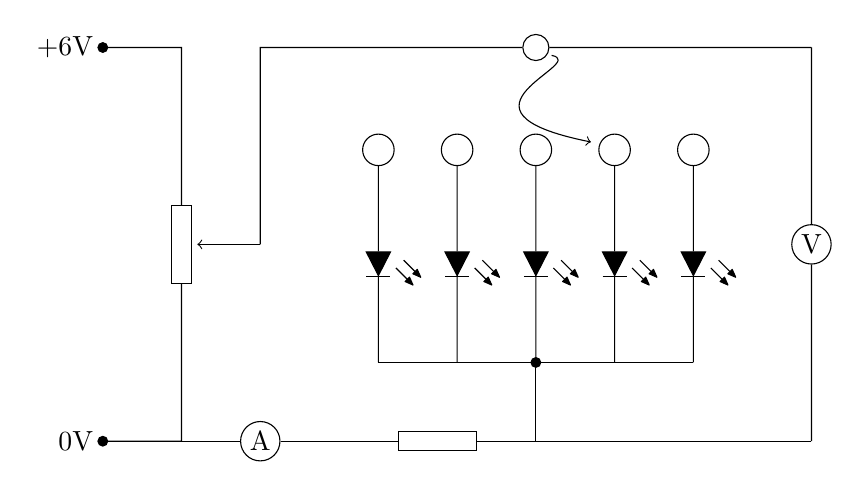
\begin{tikzpicture}[circuit ee IEC,set diode graphic=var diode IEC graphic]
\draw (0,0) node[contact]{} node[anchor=east]{\SI{0}{V}} to (1,0) to [resistor] (1,5) to (0,5) node{} node[anchor=east]{\SI{+6}{V}} node[contact]{};
\draw (0,0) to (1,0) to [circuit handle symbol={draw,shape=circle,label=center:{A},minimum size=5mm}] (3,0) node{} to [resistor] (5.5,0) node{} to (9,0);
\draw (9,0) to [circuit handle symbol={draw,shape=circle,label=center:{V},minimum size=5mm}] (9,5);
\draw (9,5) to [circuit handle symbol={draw,shape=circle,minimum size=2mm}] (2,5) to (2,2.5);
\draw[->] (2,2.5)--(1.2,2.5);
\draw (5.5,0) to (5.5,1) node[contact]{};
\draw (3.5,1) to (7.5,1);
\foreach \diode in {0,1,...,4}
{
\draw (3.5+\diode,3.5) to [diode={light emitting}] (3.5+\diode,1);
\draw (3.5+\diode,3.7) circle (0.2);
}
\draw[->] (5.7,4.9) .. controls (6.2,4.8) and (4.2,4.2) .. (6.2,3.8);
\end{tikzpicture}
\end{minipage}
\begin{minipage}{0.35\textwidth}
Some data on the LEDs from the manufacturer is below:\\

\renewcommand{\arraystretch}{1}
\begin{tabular}{lcc}
\hline
Colour & $\lambda$/nm & $I_{\text{max}}$/mA\\
\hline
Red & 700 & 25\\
Orange & 627 & 30\\
Yellow & 590 & 30\\
Green & 565 & 25\\
Blue & 430 & 30\\
\hline
\end{tabular}
\renewcommand{\arraystretch}{2}
\end{minipage}

\subsection{Measurements}
For each LED, you need to take several readings of current and voltage (which will allow you to plot a current-voltage characteristic), by increasing the voltage from zero until the current reaches the manufacturer's recommended maximum current (and no further).

\begin{minipage}{0.3\textwidth}
\begin{tabular}{|p{2cm}|p{2cm}|}
\hline
\multicolumn{1}{|c|}{$V$/V} & \multicolumn{1}{|c|}{$I$/}\\
\hline
&\\
\hline
&\\
\hline
& \\
\hline
& \\
\hline
& \\
\hline
& \\
\hline
\end{tabular}
\end{minipage}
\begin{minipage}{0.3\textwidth}
\begin{tabular}{|p{2cm}|p{2cm}|}
\hline
\multicolumn{1}{|c|}{$V$/V} & \multicolumn{1}{|c|}{$I$/}\\
\hline
&\\
\hline
&\\
\hline
& \\
\hline
& \\
\hline
& \\
\hline
& \\
\hline
\end{tabular}
\end{minipage}
\begin{minipage}{0.3\textwidth}
\begin{tabular}{|p{2cm}|p{2cm}|}
\hline
\multicolumn{1}{|c|}{$V$/V} & \multicolumn{1}{|c|}{$I$/}\\
\hline
&\\
\hline
&\\
\hline
& \\
\hline
& \\
\hline
& \\
\hline
& \\
\hline
\end{tabular}
\end{minipage}

\begin{minipage}{0.3\textwidth}
\begin{tabular}{|p{2cm}|p{2cm}|}
\hline
\multicolumn{1}{|c|}{$V$/V} & \multicolumn{1}{|c|}{$I$/}\\
\hline
&\\
\hline
&\\
\hline
& \\
\hline
& \\
\hline
& \\
\hline
& \\
\hline
\end{tabular}
\end{minipage}
\begin{minipage}{0.3\textwidth}
\begin{tabular}{|p{2cm}|p{2cm}|}
\hline
\multicolumn{1}{|c|}{$V$/V} & \multicolumn{1}{|c|}{$I$/}\\
\hline
&\\
\hline
&\\
\hline
& \\
\hline
& \\
\hline
& \\
\hline
& \\
\hline
\end{tabular}
\end{minipage}
\begin{minipage}{0.3\textwidth}
\begin{tabular}{|p{2cm}|p{2cm}|}
\hline
\multicolumn{1}{|c|}{$V$/V} & \multicolumn{1}{|c|}{$I$/}\\
\hline
&\\
\hline
&\\
\hline
& \\
\hline
& \\
\hline
& \\
\hline
& \\
\hline
\end{tabular}
\end{minipage}

\begin{questions}
\question Plot the current-voltage characteristics for all of the LEDs on the {\bf same} graph, with voltage on the $x$-axis and current on the $y$-axis (take care to label the curves!)  On this graph, you need to extrapolate each curve down to the $x$-axis to find the voltage at which current first starts to flow, and light photons start to be emitted.  Use this to fill in the table below.

\begin{center}
\begin{tabular}{|l|c|p{2cm}|p{2cm}|}
\hline
Colour & $\lambda$ &  \multicolumn{1}{|c|}{$1/\lambda$ } & \multicolumn{1}{|c|}{$V_{\text{min}}$}\\
 & / nm & \multicolumn{1}{|c|}{/ \ldots} & \multicolumn{1}{|c|}{/ V} \\
\hline
Red & 700 & &\\
\hline
Orange & 627 & &\\
\hline
Yellow & 590 & &\\
\hline
Green & 565 & &\\
\hline
Blue & 430 & &\\
\hline
\end{tabular}
\end{center}

\question Now plot a second graph, this time of the minimum voltage for light emission on the $y$-axis against the LED wavelength on the $x$-axis.

\question Work out the gradient, showing your working on the graph. \answerline

According to theory, your gradient $G$ is related to Planck's constant by $h=eG/c$, where $e$ is the electronic charge, \SI{1.6e-19}{C}, and $c$ is the speed of light, \SI{3e8}{m.s^{-1}}.

\question What value does your experiment give for $h$? \answerline

\question Comment briefly on this value, and on the quality of your data, on your second graph. What do you think were the biggest sources of error in this experiment?
\end{questions}
%graph paper incl.

\cleardoublepage

\include{prac/particles-collider}

\cleardoublepage

\section{Bubble chamber tracks}
%http://teachers.web.cern.ch/teachers/archiv/HST2005/bubble_chambers/BCwebsite/index.htm
%http://epweb2.ph.bham.ac.uk/user/watkins/seeweb/BubbleChamber.htm
\label{bubble}

In this experiment, you will determine some properties of short-lived particles by analysing photographs from a liquid hydrogen bubble chamber.  The experiment is based around measurements of film taken from the bubble chamber at CERN particle physics laboratory near Geneva.

Bubble chambers played an important part in discovering particles whose existence played an important part in establishing the quark model in the 1950s--1970s. They are no longer in use at accelerator centres, having been superseded by the faster modern electronic detectors.  However, a bubble chamber is currently being used during the search for dark matter (WIMPs).

\subsection{Background}

The bubble chamber, invented by Donald Glaser in 1952, consists of a tank of unstable (superheated) transparent liquid.  Hydrogen is often used\footnote{Hydrogen was popular as it has the simplest nucleus; other nuclei presented problems such as, `Did the beam particle hit a neutron or a proton?'}, at a temperature of about \SI{30}{K}.  This liquid is very sensitive to the passage of {\bf charged} particles, which initiate boiling as a result of the energy they deposit by ionizing the atoms as they force their way through the liquid.
Bubbles are formed along the paths of the charged particles, and these tracks of bubbles can be photographed.

\subsection{How to read bubble chamber tracks}

\begin{itemize}
\item Beam particles whose tracks do NOT remain parallel all the way through the picture must have collided with a proton in a hydrogen atom.
\item All the paths of charged particles (and we only see charged particle paths) are curved by the magnetic field.
\item Positively charged particles' paths curve one way, negatively charged particles' paths the other.  (Normally, it is not necessary to be told which way the field is pointing---the picture already contains the answer. The little curly tracks are produced by electrons which are knocked out of the atoms by charged particles passing by.)
\item The momentum of a particle is proportional to the radius of curvature of the track in the bubble chamber. 
\item When a particle has used up its energy making bubbles, it stops. So its range is a measure of its energy.  In practice, this is useful for identifying protons that have received only a gentle blow from the beam particle, thus not having enough energy to get all the way to the edge of the chamber.
\item Other particles (for example pions) may stop; but if they do, they decay in a characteristic way which tells us that they are pions. In such a case, we would know the mass $m$ and its momentum $p$ from the curvature of the track; the energy can then be calculated using: $E^{2} = p^{2}c^{2} + m^{2}c^{4}$.
\end{itemize}

So much for charged particles.  Neutral particles do NOT leave trails of bubbles.  However, we can still sometimes glean some clues about their properties:

\begin{itemize}
\item An unstable neutral particle may decay before it leaves the bubble chamber into a pair of lighter particles - one positive and one negative - leaving an easily recognizable letter V (or vee) shape.
\item If the tracks from the vee happen to cross again, downstream, the line joining the crossing position to the decay position (the V) points back to the origin of the neutral particle.
\item An uncharged particle is often produced when an unstable charged particle decays--usually into a charged particle of the same sign and one or more neutral particles. This shows up in the bubble chamber as a kink (a sudden change into a more curved track).
\item The energy and momentum of the uncharged particle(s) which leave at the kink can be inferred by conservation laws from the tracks we do see.
\item If you want to examine the picture of a collision very carefully � to find small angle kinks, for example � it is a good idea to print the picture and look at it from a very low angle.
\end{itemize}

%It is often possible to identify the kind of particle from their characteristic decay signatures.  This is a case of visual pattern recognition.

%\includegraphics[width=4cm]{sig-proton.png}

%At the LHC, where the events will have hundreds of particles in the final state, imaginative systems of electronic detectors and software have been designed to do this at incredibly high data-acquisition rates.

\subsection{Event A}


\begin{questions}
\question
\begin{parts}
\part How many charged beam particles enter the chamber? \answerline
\part In what direction is the beam moving (from the bottom to the top or vice versa)? Draw arrows on the image to show this.
\part If there are any knock-on electrons, label these on the image.
%\part What is the direction of the magnetic field? \answerline
\part How many collisions do you see? \answerline
\part How many particles result from each of the collisions? \answerline
\part Identify the charges of these particles, and explain your reasoning. \fillwithlines{2cm}
\part What is the charge of the beam particles (assuming collisions are with protons)? \answerline
\part How many kinks do you see?\answerline
\part How many vees do you see? \answerline
\part How many particles result from the decays? \answerline
\part Identify the charges of the particles from decays, and explain your reasoning. \fillwithlines{2cm}
\part Consider the main collision/interaction. Which of the charged particles from the collision has the lowest momentum? How do you know?\fillwithlines{3cm}
\end{parts}

\includegraphics[width=0.7\textwidth]{img/event_Agal3_kzero11.png}\\
{\footnotesize Event A.  The crosses are known as fiducials and are marked at positions which are accurately surveyed. They are measured along with events and are essential to the 3D reconstruction process.} %(From the Latin word `fiducia' meaning truth.)}

\subsection{Event B}
\includegraphics[width=0.7\textwidth]{img/event_Bgal2_231.png}\\

\begin{parts}
\part In what direction is the beam going?  Mark this with an arrow on the photograph.
\part How many beam tracks are there? \answerline
\part How many collisions are there? \answerline
\part How many vees are there? \answerline 
\part How many kinks are there? \answerline
\part What does the fact that you see a track indicate? \fillwithlines{1cm}
\part How can you tell if two tracks represent particles of the opposite charge?\fillwithlines{2cm}
\part What physical property of a particle is determined by the curvature of its track?\answerline
\part What causes a kink?\fillwithlines{2cm}
\part What causes a vee?\fillwithlines{2cm}
\part What are the small crosses?\fillwithlines{1cm}
\part What is the charge of the target particles (remember this is a hydrogen bubble chamber)? \answerline
\part What is the charge of the beam and how do you know? \fillwithlines{1cm}
\part In which direction are the neutral particle(s) moving from the kinks? \fillwithlines{1cm}
\part What needs to happen for a track to kink twice? \fillwithlines{2cm}
%\part How does the difference in mass between the initial state (before the kink) and the final state (after the kink) affect the angle of the kink?
\part What particles can cause a vee? \fillwithlines{1cm}
\part From which point do the particles that cause the vees come? \fillwithlines{1cm}
\end{parts}


\subsection{Event C}
\begin{parts}
\part How many charged beam particles enter the chamber? \answerline
\part In what direction is the beam moving (from the bottom to the top or vice versa)?  Put an arrow on the photograph to show this.
\part Are there any knock-on electrons? If so, label these on the photograph.
%\part What is the direction of the magnetic field (assuming the targets are protons)?
\part How many collisions do you see? \answerline
\part How many particles result from each of the collisions? \fillwithlines{1cm}
\part Identify the charges of these particles.\fillwithlines{2cm}
\part What is the charge of the beam particles? How do you know? \fillwithlines{2cm}
\part How many kinks do you see? \answerline
\part How many vees do you see? \answerline
\part How many particles result from the decays? \fillwithlines{2cm}
\part Identify the charges of the particles from decays.\fillwithlines{3cm}
\part Identify the possibilities particle that decays, forming a vee.\fillwithlines{2cm}
\part Identify the possibilities for the particle that decays, forming a kink.\fillwithlines{2cm}
\end{parts}
\end{questions}
\includegraphics[width=0.7\textwidth]{img/event_Cgal3_omega_1.png}



\cleardoublepage

%\include{prac/especificq-bcircles}

%\cleardoublepage

%\include{prac/gammaabsorption}

%\include{res/graphpaper}

%\cleardoublepage

%\include{res/graphpaper}

%\cleardoublepage

%\include{prac/radioactivityanalogue}

%\include{res/graphpaper}

%\cleardoublepage



\end{document}

%%%%%%%%%%%%%%%%%%%%%%%%%%%%%%%%%%%%%%%%%%%%%%%%%%%%%%%%%%%%%%%%%%%%%%%%%%%%%%%%%%%%%%%%%%
% SOME MORE IDEAS FOR UNIT 1 PRACTICALS BELOW!
%%%%%%%%%%%%%%%%%%%%%%%%%%%%%%%%%%%%%%%%%%%%%%%%%%%%%%%%%%%%%%%%%%%%%%%%%%%%%%%%%%%%%%%%%%
%
%%%%%%%%%%%%%%%%%%%%%%%%%%%%%%%%%%%%%%%%%%%%%%%%%%%%%%%%%%%%%%%%%%%%%%%%%%%%%%%%%%%%%%%%%%

\subsection{Momentum conservation}
The first activity is to verify, using bubble chamber tracks, that momentum conservation is obeyed in collisions of subatomic particles.
The actual experiment took place at CERN in the mid 1970s with incident protons of a momentum \SI{2}{GeV/$c$}.
The bubble chamber photograph shows an elastic collision between a proton entering from the left, and a (more-or-less) stationary proton in a hydrogen-filled bubble chamber.

Students can measure the radii r of the paths followed by the protons, using this template of curves provided (click here), and since momentum p is directly proportional to r (click here), they can construct a vector diagram to verify that p = p1 + p2 within the errors of the method. 

\section{Cloud chamber}
\label{cloud}

The cloud chamber was invented by C.T.R. Wilson, a physicist at Cambridge University, in 1911, and won the Nobel prize in physics in 1927 for its development.  It played a prominent role in experimental particle physics until the bubble chamber was invented in the 1950s, and the discoveries of the positron in 1932 and the kaon in 1953 were made using cloud chambers as detectors.

In the chamber, conditions for cloud formation are created by cooling a saturated vapour until it is slightly supersaturated.  This means that it is cool enough for droplets to grow, but not cool enough for the droplets to form spontaneously, and it is very sensitive to anything which might make forming a droplet slightly easier. When an ionizing particle passes through the chamber, it will tend to crash into a series of molecules leaving a number of charged ions.  The vapour then starts to condense on these ions, and this is where droplets will form and grow.  This means that in the wake of the ionizing particles a line of droplets - a thin cloud trail - is formed allowing you to see their paths (rather like that behind a jet aircraft in an otherwise clear sky).

The cloud chamber you will use is slightly different from Wilson's original design.  It was devised in 1939 by Alexander Langsdorf, and is known as a diffusion cloud chamber.  In this design, the bottom of the chamber is cooled to a rather low temperature, and the vapour is introduced from the top of the chamber.  The vapour cools as it falls, until at some level it starts to condense, forming a cloud of alcohol droplets which fall down to the plate at the bottom.  Just above the point where the droplets are forming naturally there is an area of supersaturated vapour.  This region is where the ionizing particle tracks are formed, and particles are detected.

%Diagram

%Instructions on getting it to work

%http://www.practicalphysics.org/go/Experiment_584.html?topic_id=40&collection_id=78

%Questions

\section{Particle Physics Detector}
\texttt{lppp.ac.uk}

%already available on website. Select suitable material and questions.

\section{Line spectra}

% need diffraction theory
